%=========================================================================%
%   LaTeX File for Master thesis of Sun Yat-Sen University
%-------------------------------------------------------------------------%
%   Copyright 2004  by      (FBI@BHQT)
%-------------------------------------------------------------------------%
%   Latex 硕士论文模板
%   在ctex2.3.3(miktex2.3)、ctex2.4.6完全安装下通过测试.
%   本模板使用ctex.org的cjk版本
%   -- 经刘成明根据大连理工大学研究生院2007-6-5发布的博士学位论文模板修改而成。
%      2008年5月8日根据中山大学研究生院最新模板修订。
%   -- 2009年4月经车春回根据刘成明老师的博士论文模板修改而成,符合中山大学硕士
%      硕士研究生要求。
%=========================================================================%

\documentclass[12pt,openany,a4paper,twoside]{mybook}
%algorithm和algorithmic这两个宏包用于画伪代码
%\usepackage{algorithm}
%\usepackage{algorithmic}
%使用booktab宏包定义三条划线命令:\toprule、\midrule 和 \bottomrule
%用于画三线表
\usepackage{booktabs}
\usepackage{amsmath,amssymb}

%=========================================================================%
%                          引用的宏包和相应的定义
%\usepackage{overcite}
%\usepackage[super]{natbib}
%=========================================================================%

%============================ 中文支持宏包 ==============================%
\usepackage[BoldFont,SlantFont]{xeCJK}
\usepackage{CJKnumb}
%====================== 图形和超链接支持宏包 ========================%
\usepackage[CJKbookmarks=true,
            bookmarksnumbered=true,
            bookmarksopen=true,
            colorlinks=true, %注释掉此项则交叉引用为彩色边框(将colorlinks和pdfborder同时注释掉)
            pdfborder=001,   %注释掉此项则交叉引用为彩色边框
            citecolor=blue,%
            linkcolor=blue
            ]{hyperref}

\usepackage{booktabs}
\usepackage{amsmath,amssymb}

\usepackage[numbers,sort&compress]{natbib}
\usepackage{color}              % 支持彩色
\usepackage{subfigure}          % 支持子图
\usepackage{floatflt}           % 图文混排用宏包
\usepackage{rotating}           % 图形和表格的控制
\usepackage{flafter}            % 因为图形可浮动到当前页的顶部,所以它可能会出现
                                % 在它所在文本的前面. 要防止这种情况,可使用 flafter
                                % 宏包
\usepackage[below]{placeins}    %浮动图形控制宏包
                                %允许上一个section的浮动图形出现在下一个
                                %section的开始部分该宏包提供处理浮动对象
                                %的 \FloatBarrier 命令,使所有未处理的浮动
                                %图形立即被处理
%\usepackage{endfloat}          %可将浮动对象放置到文件的最后
%\usepackage{overpic}           %将LaTeX对象放置在图上
%\usepackage{pstricks}          %Postscript macrosfor Generic TeX(我没用过,据说很强)
%\usepackage{bez123}
%============================表格支持宏包=================================%
\usepackage{rotating}   % 用法 \begin{sidewaystable}....\end{sidewaystable}
                        % 即可旋转表格
\usepackage{longtable}  % 支持长表格
\usepackage{tabls}
\usepackage{multirow}   % 表格多行合并, 矩阵的边注
\usepackage{colortbl}   % 彩色表格
\usepackage{dcolumn}    % 让表格中将小数点对齐
\usepackage{hhline}     % 在表格中用 \hhline 得到的结果就如同\hline
                        % 或 \hline\hline,当然在和垂直线的交叉处会有所不同。
\usepackage{slashbox}   % 可在表格的单元格中画上一斜线。

%\newcommand{\centpcol}{\leftskip\fill \rightskip\fill}%制表使可用p{ncm}设置栏宽,还使本栏居中

%\iffalse 举例
%  \begin{tabular}{|l|c|c|} \hline
%    & \multicolumn{2}{c|}{MRD} \\ \cline{2-3}
%   & \multicolumn{1}{p{3.5cm}|}{\centpcol Same as previous response} &
%     \multicolumn{1}{p{3.5cm}|}{\centpcol Different from previous response}\\
%   \hline
%    Observed frequency & 966 & 148 \\
%    Expected frequency & 1066 & 48 \\ \hline
%    \multicolumn{3}{c}{${\chi}^2 = 213.97,\quad \mathit{d.f.}=1,\quad p<0.001$}
%  \end{tabular}
%\fi

%============================版面控制宏包=================================%
%\usepackage[top=1.7cm,bottom=2cm,left=2.5cm,right=2.1cm,includehead,includefoot]{geometry}                 % 页面设置
\usepackage[top=3.5cm,bottom=3.5cm,left=2.5cm,right=2.5cm,includefoot]{geometry}%定制页面大小

%---------------------------16开纸张大小页面设置--------------------------------%
%16开不是标准的西式纸张大小,比a4,letter小,比b5稍大.可以通过使用anysize宏包实现:
%可以很好的解决在PdFLaTeX下纸张大小问题;但不能很好解决,LaTeX以及DVI2PDF下的问题
%请注意\documentclass[]{book}%中不要指明诸用a4paper之类的选项, 其他选项无所谓.
%若要用16开纸请将下列\iffalse \fi 注释掉
\iffalse
\usepackage{anysize}
%\papersize{height}{width}%设置页面的大小。这个命令可以不用,因为缺省可在%\documentclass选项中设定标准得页面大小。一般为a4paper。
\papersize{26cm}{18.4cm}
%\marginsize{left}{right}{top}{bottom}%{}中指的是各边界的margin,对于像book等双面版式来说,这里的left和right在奇偶页会互换。
\marginsize{2.5cm}{2.1cm}{2cm}{2cm}
\fi

\usepackage{indentfirst}                 %  首行缩进宏包
\usepackage[perpage,symbol]{footmisc}    %  脚注控制
\usepackage{fancyhdr}                    %  fancyhdr宏包 页眉和页脚的相关定义
\usepackage{lastpage}                    % 自动记录总页数宏包,计数器为 LastPage
                                         % 注意大小写
\usepackage{pageno}                      % 章首页的页眉处理, 可以改为自己想要的形式
%\iffalse \makeatletter
%\renewcommand{\ps@plain}{%
%   \renewcommand{\@mkboth}{\@gobbletwo}%
%   \renewcommand{\@evenhead}{\reset@font\sf -- \thepage -- \hfil}%
%   \renewcommand{\@oddhead}{\reset@font\sf\hfil -- \thepage --}%
%   \renewcommand{\@evenfoot}{}%
%   \renewcommand{\@oddfoot}{}
%} \makeatother \fi

%======================= 多列文本与多列编号宏包 ===========================%
\usepackage{multicol,multienum}
%\iffalse 用法为:可嵌套使用
%\begin{multienumerate}[evenlist,oddlist]
%\mitemxxxx{Not}{Linear}{Not}{Quadratic}
%\mitemxxxo{Not}{Linear}{No; if $x=3$, then $y=-2$.}
%\mitemxx{$(x_1,x_2)=(2+\frac{1}{3}t,t)$ or
%$(s,3s-6)$}{$(x_1,x_2,x_3)=(2+\frac{5}{2}s-3t,s,t)$}
%\end{multienumerate}
%\begin{multicols}{2}
%\end{multicols}
%\fi

%======================== 数学公式相关宏包 ===============================%
\usepackage{bm}         % 处理数学公式中的黑斜体的宏包
\usepackage{amsmath}    % AMSLaTeX宏包 用来排出更加漂亮的公式
\usepackage{amssymb}    % AMSLaTeX宏包 用来排出更加漂亮的公式
%\usepackage{mathrsfs}  % 不同于\mathcal or \mathfrak 之类的英文花体字体
\usepackage[amsmath,thmmarks]{ntheorem} % 定理类环境宏包,其中 amsmath 选项
                                        % 用来兼容 AMS LaTeX 的宏包
\usepackage{subeqnarray} %多个子方程(1-1a)(1-1b)
%\iffalse 以下是一个例子
%\begin{subeqnarray}
%\label{eqw} \slabel{eq0}
% x & = & a \times b \\
%\slabel{eq1}
% & = & z + t\\
%\slabel{eq2}
% & = & z + t
%\end{subeqnarray}
%\fi

%=============================标题与列表宏包=============================%
\usepackage[sf]{titlesec}   % 控制标题的宏包,配合命令在后面,
                            % 将cjk+miktex+scrbook+gb.cap下的章的标题号,
                            % 比如~``第二章 XXX''位置于中心

\usepackage{titletoc}     %定制目录的宏包
%\usepackage{hyperref}
%\usepackage[super,sort&compress,numbers]{natbib}  % 支持引用的宏包
%\usepackage{hypernat}
\newcommand{\supercite}[1]{\textsuperscript{\cite{#1}}}
\usepackage{enumerate}      % 改变列表标号样式宏包 其后可接选项[a,A,i,I,1]
\usepackage{ccaption}\captiondelim{\ }       % 浮动图形和表格标题样式,可选项为
                            % [scriptsize,footnotesize,centerlast]
%\usepackage{setspace}      % 图形和表格的标题如果是多行,行距比较大,可以加宏包
\usepackage{pifont}         % 有很漂亮的带圈的各种数字符号使用
%\usepackage{atbeginend}    % 可选宏包, 能解决许多问题,
                            % 比如itemize, enumerate环境\item之间的控制
%用法
%\AfterBegin{itemize}{\addtolength{\itemsep}{-0.5\baselineskip}}
%\AfterBegin{enumerate}{\addtolength{\itemsep}{-0.5\baselineskip}}

\iffalse
%=================== 支持LaTexCAD生成的源程序的宏包 =====================%
\usepackage{TEXcad/lgrind}     % for formated source code
\usepackage{TEXcad/latexcad}   % latexcad.sty for drawings etc
\usepackage{TEXcad/epic}       %picture macros
\usepackage{TEXcad/eepic}      %extended picture macros
\usepackage{TEXcad/fancybox}   %box macros
\usepackage{TEXcad/epsf}       %postscript macros
\usepackage{TEXcad/rotate}     % postscript text rotation macros


%=========================== 特殊文本元素宏包 ==============================%
\usepackage{nicefrac}   % 在正文文本中排版分式时,可以用它来得到较好的排版效果。
\usepackage{units}      % 基于 nicefrac 宏包,提供对计量单位比较美观的排版效果。
\usepackage{soul}       % 支持对单词加上下划线或其每个字母在一定的宽度内均匀散布
\usepackage{altfont}    % 使用该宏包, 可以在一个宏包中使用多种不同的字体,
                        % 包括PSNFSS 和 MFNFSS
%\usepackage{prelim2e}  % 可以在每页页脚下方标记出本文档的版本信息等
\usepackage{a0size}     %自由定义字号,在后面“字号设置”中可设置到107pt为止的大字体
\fi

%=================================源代码宏包================================%
\usepackage{listings}

%=================================建立索引宏包================================%
\usepackage{makeidx}
\makeindex

%*******************自定义计数器,统计论文总页表格数,插图数*************************
\newcounter{totalfig}           %***在正文含有表或图的每章chapter开始前,加上如下两句
\newcounter{totaltab}           %***\addtocounter{totalfig}{\value{figure}}
                                %***\addtocounter{totaltab}{\value{table}}

\newcommand{\ctex}{C\TeX}

%=========================================================================%
%   LaTeX File for PhD thesis of Dalian University of Technology
%-------------------------------------------------------------------------%
%   Copyright 2003  by     (FBI@BHQT)
%=========================================================================%

%=========================================================================%
%                          主文档 格式定义
%=========================================================================%

%===================== 重定义字体、字号命令 =============================%
% 注意win2000,没有 simsun, 最好到网上找一个。一些字体是office2000带的
\setCJKmainfont{SimSun}

\setCJKfamilyfont{hei}{SimHei}
\newcommand{\hei}{\CJKfamily{hei}}                          %黑体
\setCJKfamilyfont{kai}{KaiTi}
\newcommand{\kai}{\CJKfamily{kai}}                          %行楷
\setCJKfamilyfont{fang}{FangSong}
\newcommand{\fang}{\CJKfamily{fang}}                        %仿宋
\setCJKfamilyfont{song}{SimSun}
\newcommand{\song}{\CJKfamily{song}}                        %宋体 song
%\setCJKfamilyfont{xingkai}{FZXingKai-S04}
%\newcommand{\xingkai}{\CJKfamily{xingkai}}                  %华文行楷



\newcommand{\chuhao}{\fontsize{42pt}{\baselineskip}\selectfont}     % 字号设置
\newcommand{\xiaochuhao}{\fontsize{36pt}{\baselineskip}\selectfont} % 字号设置
\newcommand{\xiaoyi}{\fontsize{24pt}{\baselineskip}\selectfont}     % 小一, 单倍行距
\newcommand{\yihao}{\fontsize{28pt}{\baselineskip}\selectfont}      % 字号设置
\newcommand{\erhao}{\fontsize{21pt}{\baselineskip}\selectfont}      % 字号设置
\newcommand{\xiaoerhao}{\fontsize{18pt}{\baselineskip}\selectfont}  % 字号设置
\newcommand{\sanhao}{\fontsize{15.75pt}{\baselineskip}\selectfont}  % 字号设置
\newcommand{\xiaosanhao}{\fontsize{15pt}{\baselineskip}\selectfont} % 字号设置
\newcommand{\sihao}{\fontsize{14pt}{\baselineskip}\selectfont}      % 字号设置
\newcommand{\xiaosihao}{\fontsize{12pt}{\baselineskip}\selectfont}  % 字号设置
\newcommand{\wuhao}{\fontsize{10.5pt}{\baselineskip}\selectfont}    % 字号设置
\newcommand{\xiaowuhao}{\fontsize{9pt}{\baselineskip}\selectfont}   % 字号设置
\newcommand{\liuhao}{\fontsize{7.875pt}{\baselineskip}\selectfont}  % 字号设置
\newcommand{\qihao}{\fontsize{5.25pt}{\baselineskip}\selectfont}    % 字号设置

%===================================================================%
%                         各种距离与缩进
%===================================================================%

%-------------------- 用于中文段落缩进 和正文版式 ------------------%

\setlength{\parindent}{2em}                 % 首行两个汉字的缩进量
\setlength{\parskip}{3pt plus1pt minus1pt}  % 段落之间的竖直距离
\renewcommand{\baselinestretch}{1.25}\normalsize      % 定义行距

%------------------------- 列表与图表距离设置 -----------------------%
\setlength{\topsep}{3pt plus1pt minus2pt}           % 第一个item和前面版落间的距离
\setlength{\partopsep}{3pt plus1pt minus2pt}        % 当在一个新页开始时加到
                                                    % \topsep的额外空间
\setlength{\itemsep}{3pt plus1pt minus2pt}          % 连续items之间的距离.
\setlength{\floatsep}{10pt plus 3pt minus 2pt}      % 图形之间或图形与正文之间的距离
\setlength{\abovecaptionskip}{2pt plus1pt minus1pt} % 图形中的图与标题之间的距离
\setlength{\belowcaptionskip}{3pt plus1pt minus2pt} % 表格中的表与标题之间的距离

%下面这组命令使浮动对象的缺省值稍微宽松一点,从而防止幅度
%对象占据过多的文本页面,也可以防止在很大空白的浮动页上放置
%很小的图形。
\renewcommand{\textfraction}{0.15}
\renewcommand{\topfraction}{0.85}
\renewcommand{\bottomfraction}{0.65}
\renewcommand{\floatpagefraction}{0.60}

%---------------------------- 数学公式设置 ------------------------------%
\setlength{\abovedisplayskip}{5pt plus1pt minus1pt}     %公式前的距离
\setlength{\belowdisplayskip}{5pt plus1pt minus1pt}     %公式后面的距离
\setlength{\arraycolsep}{2pt}   %在一个array中列之间的空白长度, 因为原来的太宽了

\allowdisplaybreaks[4]  % \eqnarray如果很长,影响分栏、换行和分页
                        %(整块挪动,造成页面空白),可以设置成为自动调整模式

\renewcommand{\mathbf}[1]{\boldsymbol{#1}}  %重新定义 \mathbold 为矢量黑斜体
                                            %用Mathtype生成的公式源码直接应用于程序中
                                            %(导出时请选择 TeX-AMS-LaTeX )

\newcommand{\me}{\mathrm{e}}  %定义 对数常数e,虚数符号i,j以及微分算子d为直立体。
\newcommand{\mi}{\mathrm{i}}
\newcommand{\mj}{\mathrm{j}}
\newcommand{\dif}{\mathrm{d}}

%===================================================================%
%                         各种标题样式
%===================================================================%
%======================= 标题名称中文化 ============================%
\renewcommand\contentsname{目\ 录}
\renewcommand\listfigurename{插\ 图\ 目\ 录}
\renewcommand\listtablename{表\ 格\ 目\ 录}
%\renewcommand\abstractname{摘\ 要} %err undefined
%\renewcommand\refname{参考文献}         %article类型
%\renewcommand\bibname{\song\sanhao{\textbf{参\ 考\ 文\ 献}}}    %book类型
\renewcommand\indexname{索\ 引}
\renewcommand\figurename{图}
\renewcommand\tablename{表}
\renewcommand\partname{第\CJKnumber{\value{part}}部分}
\renewcommand\chaptername{第\CJKnumber{\value{chapter}}章}
%\renewcommand\chaptername{\CJKprechaptername\CJKthechapter\CJKchaptername}
%======================= 定制章节的标题样式 =============================%
\setcounter{secnumdepth}{3}
%---------------------- 定义章节的编号格式 --------------------------%
%\renewcommand{\thesection}{\CJKnumber{\arabic{section}}、} % 定义 一、。九、十
\renewcommand{\thesection}{\arabic{chapter}.\arabic{section}}
\renewcommand{\thesubsection}{\arabic{chapter}.\arabic{section}.\arabic{subsection}}
\renewcommand{\thesubsubsection}{\arabic{subsubsection}.}
\let\oldtitle=\title
\def\title#1{\oldtitle{\cnbf{#1}}}

%\CJKtilde   %用于解决英文字母和汉字的间距问题。例如:变量~$x$~的值。
            %这个命令重新定义~。等价于 \def~{\hspace{0.25em plus 0.125em minus 0.08em}}
            %若想恢复~,则用命令 \standardtilde 。

\renewcommand{\CJKglue}{\hskip 0pt plus 0.08\baselineskip}
%\CJKglue   %这个命令原始定义为
            %newcommand{\CJKglue}{\hskip 0pt plus 0.08\baselineskip}
            %它于必要时在汉字之间插入一个附加的空隙,以解决行的超长问题。
            %可以修改此命令,增加它的值,以加强其调节能力。
            %注意,使用这个命令可能导致出现空白页!!!

%----------------------- 定义章节标题格式 ----------------------------%

%\titleformat{\chapter}[hang]{\xiaoerhao\filcenter\CJKfamily{hei}\Large}
%        {\Large \chaptertitlename}{10em}{}{}
\titleformat{\chapter}[hang]{\normalfont\sanhao\filcenter\CJKfamily{hei}}
    {\sanhao{\chaptertitlename}}{20pt}{\huge}
\titlespacing{\chapter}{0pt}{-3ex  plus .1ex minus .2ex}{2.5ex plus .1ex minus .2ex}

%\titleformat{\section}[hang]{\CJKfamily{hei}\Large \centering} %标题居中
\titleformat{\section}[hang]{\sanhao\CJKfamily{hei}}
    {\sihao\thesection}{1em}{}{}
\titlespacing{\section}
    {0pt}{1.5ex plus .1ex minus .2ex}{\wordsep}

\titleformat{\subsection}[hang]{\sihao\CJKfamily{hei}}
    {\sihao\thesubsection}{1em}{}{}
\titlespacing{\subsection}%
    {0pt}{1.5ex plus .1ex minus .2ex}{\wordsep}

\titleformat{\subsubsection}[hang]{\CJKfamily{hei}}
    {\thesubsubsection }{1em}{}{}
\titlespacing{\subsubsection}%
    {0pt}{1.2ex plus .1ex minus .2ex}{\wordsep}

%======================= 定义列表项目格式 ==========================%
\renewcommand\labelenumi{\textcircled{\scriptsize \theenumi}}  %带圈的数字
%\renewcommand\labelenumi{(\theenumi)}
\renewcommand\labelenumii{(\theenumii)}
\renewcommand\labelenumiii{\theenumiii.}
\renewcommand\labelenumiv{\theenumiv.}

%====================== 定制图形和表格标题样式 =====================%
%---------------------- 定制图形和表格标题格式 ---------------------%
\renewcommand{\captiondelim}{\ } %定义如  "图(表)2: 示例" 中的间隔符号,如 ":" ,这里定义为空
%\renewcommand{\captionlabelsep}{\hspace{1em}} %定义图表编号与标题间的间隔距离
%\renewcommand{\captionlabelfont}{\small \CJKfamily{hei}\bf} %定义图表标签的字体
%\renewcommand{\captionfont}{\small \CJKfamily{song}\rmfamily} %定义图表标题内容的字体
%% \scriptsize \footnotesize \small \large \Large  %图形标签字体大小


%--------------------- 定义图、表、公式的编号格式 -------------------%
\renewcommand{\thetable}{\arabic{chapter}-\arabic{table}}
%\renewcommand{\theequation}{\arabic{chapter}-\arabic{equation}}
\renewcommand{\thefigure}{\arabic{chapter}-\arabic{figure}}


%=========================== 目录设置 ==================================%
\setcounter{tocdepth}{2} \setcounter{secnumdepth}{2}
% 可以用\section[abc]{abcdefg}形式的命令,这样abc就做为缩短标题出现
% 在目录表中和页眉上.另外,还可以利用\addtocounter{secnumdepth}{num}
% 来使得当前章节编号深度增加或减小,num可取正值或负值.
%*******取自ctex           定义目录格式   启用titletoc宏包
%%******序号,标题间距等
\titlecontents{chapter}[2.em]{\color{black}\normalsize}%\CJKfamily{hei}\addvspace{4ex}}
 {\contentslabel{2em}\hspace*{1.0em}}{\hspace*{-2.3em}}
 {\color{black}\titlerule*[0.4pc]{.}\contentspage}[\addvspace{0.5ex}]

\titlecontents{section}
[3.4em] {\color{black}\normalsize}
{\contentslabel{2em}\hspace*{-0.0em}} {\hspace*{-2.3em}}
{\color{black}\titlerule*[0.4pc]{.}\contentspage}

\titlecontents{subsection}
[5.4em] {\color{black}\normalsize}
{\contentslabel{2em}\hspace*{1.0em}} {\hspace*{-3.3em}}
{\color{black}\titlerule*[0.4pc]{.}\contentspage}
%%%%%%%%%%%%%%%%%%%%%%%%%%%%%%%%%%%%%%%%%%%%%%%%%%%%%%

%  缩小目录中各级标题之间的缩进
%\dottedcontents{chapter}[1.0em]{\hei\vspace{0.1em}}{1.0em}{5pt}
%\dottedcontents{section}[2.2cm]{}{2.5em}{5pt}
%\dottedcontents{subsection}[3.0cm]{}{2.5em}{5pt}
%\dottedcontents{subsubsection}[2.86cm]{}{3.4em}{5pt}


%============================= 页面设置 ================================%
%-------------------- 定义页眉和页脚 使用fancyhdr 宏包 -----------------%
% 定义页眉与正文间双隔线
\iffalse
\newcommand{\makeheadrule}{%
    \makebox[-3pt][l]{\rule[.7\baselineskip]{\headwidth}{0.4pt}}
    \rule[0.85\baselineskip]{\headwidth}{1.5pt}\vskip-.8\baselineskip}
\makeatletter
\renewcommand{\headrule}{%
    {\if@fancyplain\let\headrulewidth\plainheadrulewidth\fi
     \makeheadrule}}
\makeatother
\fi

%**************重定义在页眉处画一单横线
\newcommand{\makeheadrule}{%
    \makebox[-3pt][l]{\rule[0.7\baselineskip]{\headwidth}{0.4pt}}}
%    \rule[0.85\baselineskip]{\headwidth}{1.5pt}\vskip-.8\baselineskip}
\makeatletter
\renewcommand{\headrule}{%
    {\if@fancyplain\let\headrulewidth\plainheadrulewidth\fi
     \makeheadrule}}
\makeatother

%如果需要画单隔线,则需要
\iffalse%-------------------------------%
\renewcommand{\headrulewidth}{0.5pt}    %在页眉下画一个0.5pt宽的分隔线
\renewcommand{\footrulewidth}{0pt}      % 在页脚不画分隔线。
\fi%-------------------------------------%

\pagestyle{fancyplain}

\renewcommand{\chaptermark}[1]%
{\markboth{\chaptername \ #1}{}}            % \chaptermark 去掉章节标题中的数字
\renewcommand{\sectionmark}[1]%
{\markright{\thesection \ #1}{}}            % \sectionmark 去掉章节标题中的数字
\fancyhf{}  %清除以前对页眉页脚的设置

\fancyhead[CO]{\color{black}\CJKfamily{song}\wuhao\ctitle\hfill\leftmark}     % 在book文件类别下,
\fancyhead[CE]{\color{black}\CJKfamily{song}\wuhao\ctitle\hfill\leftmark}     % \leftmark自动存录各章之章名,
%\fancyhead[C]{\color{blue}\CJKfamily{fs}{\mytitle}}       %此处替换论文的题目
%\fancyfoot[L]{\CJKfamily{fs}hdwyn@sohu.com}             % \rightmark记录节标题
\fancyfoot[C]%                                          % [RE][LO]
{\CJKfamily{hei} -~\thepage~-}
%{\CJKfamily{hei} 第\thepage页,共\pageref{LastPage}页}
%\fancyfoot[R]{\CJKfamily{fs}学位论文模板}

%如果要要改变封面和章首页的页眉和页脚,则需要
\iffalse%----------------------------------------%
\fancypagestyle{plain} {
\fancyhead{}                                    % clear all header fields
\fancyhead[CE,CO]{这是章首页或封面的页眉}
\renewcommand{\headrulewidth}{0pt}
\fancyfoot{}                                    % clear all footer fields
\fancyfoot[CE,CO]{\thepage} }
\fi%--------------------------------------------%

%=== 配合前面的ntheorem宏包产生各种定理结构,重定义一些正文相关标题 ===%
\theoremstyle{plain}
\theoremheaderfont{\normalfont\rmfamily\CJKfamily{hei}}
%\theorembodyfont{\normalfont\rm\CJKfamily{song}} \theoremindent0em
\theorembodyfont{\normalfont\rm\CJKfamily{kai}} \theoremindent0em
\theoremseparator{\hspace{1em}} \theoremnumbering{arabic}
%\theoremsymbol{}          %定理结束时自动添加的标志
\newtheorem{definition}{\hspace{2em}定义}[chapter]
%\newtheorem{definition}{\hei 定义}[section] %!!!注意当section为中国数字时,[sction]不可用!
\newtheorem{proposition}{\hspace{2em}命题}[chapter]
\newtheorem{property}{\hspace{2em}性质}[chapter]
\newtheorem{lemma}{\hspace{2em}引理}[chapter]
%\newtheorem{lemma}[definition]{引理}
\newtheorem{theorem}{\hspace{2em}定理}[chapter]
\newtheorem{axiom}{\hspace{2em}公理}[chapter]
\newtheorem{corollary}{\hspace{2em}推论}[chapter]
\newtheorem{claim}{\hspace{2em}断言}[chapter]
\newtheorem{exercise}{\hspace{2em}习题}[chapter]
\theoremsymbol{$\blacksquare$}
\newtheorem{example}{\hspace{2em}例}[chapter]

\theoremstyle{nonumberplain}
\theoremheaderfont{\CJKfamily{hei}\rmfamily}
\theorembodyfont{\normalfont \rm \CJKfamily{song}}
\theoremindent0em \theoremseparator{\hspace{1em}}
\theoremsymbol{$\blacksquare$}
\newtheorem{proof}{\hspace{2em}证明}
\newtheorem{branchrule}{\hspace{2em}分支规则}

%=========================== 修改引用的格式 ==============================%
% 第一行在引用处数字两边加方框
% 第二行去除参考文献里数字两边的方框
%\makeatletter
%\def\@cite#1{\mbox{$\m@th^{\hbox{\@ove@rcfont[#1]}}$}}
%\renewcommand\@biblabel[1]{#1}
%\makeatother
% 增加 \upcite 命令使显示的引用为上标形式
%\newcommand{\upcite}[1]{$^{\mbox{\scriptsize \cite{#1}}}$}             % 方法1
\newcommand{\upcite}[1]{\textsuperscript{\textsuperscript{\cite{#1}}}}  % 方法2
%\makeatletter
%\def\@cite#1#2{\textsuperscript{[{#1\if@tempswa,#2\fi}]}}
%\makeatother
%=============================== 脚注 =============================%
\renewcommand{\thefootnote}{\arabic{footnote}}
%detcounter{footnote}{0}

%==================== 定义题头格言的格式 ==========================%
% 用法 \begin{Aphorism}{author}
%         aphorism
%      \end{Aphorism}
\newsavebox{\AphorismAuthor}
\newenvironment{Aphorism}[1]
{\vspace{0.5cm}\begin{sloppypar} \slshape
\sbox{\AphorismAuthor}{#1}
\begin{quote}\small\itshape }
{\\ \hspace*{\fill}------\hspace{0.2cm} \usebox{\AphorismAuthor}
\end{quote}
\end{sloppypar}\vspace{0.5cm}}

%============================== 控制表格线宽 ==========================%
% 更改横线(\hline)线宽:定义如下命令\hlinewd代替\hline。
% 更改垂直线(\vline)线宽:使用\usapackage{array},则可以在指定垂直线的地方用
% “!{\vrule width 3.5pt}”代替“|”,如“|c!{\vrule width 5pt}p{5cm}|r|”

\makeatletter
\def\hlinewd#1{%
  \noalign{\ifnum0=`}\fi\hrule \@height #1 \futurelet
   \reserved@a\@xhline}
\makeatother
\newcommand\vlinewd[1][1pt]{\vrule width #1}

% 不过上面的命令\hlinewd不能与longtable正常工作(reported by %钟圣俊老师),
% 只能使用下面的方法实现线宽控制:
%
%\setlength{\arrayrulewidth}{0.5pt}
%\setlength{\doublerulesep}{\arrayrulewidth}
%\newcommand{\dhline}{\hline\hline}
%\newcommand{\thline}{\hline\hline\hline}
%(类似的可以定义更多不同宽度的\hline)


%========================== 其它自定义 ==============================%
%====================================================================%
% 下面定义的命令(\alpheqn \reseteqn)可以使公式编号变为 4-a,4-b
% 使用说明:\alpheqn 为开始产生处,\reseteqn为恢复原来公式编号形式处
% 这两个命令为自定义,使用时应注意:不可放于 数学环境中!!!
% 在公式开始前和结束后使用!!!
%====================================================================%
%\newcounter{saveeqn}%
%
%\newcommand{\alpheqn}{%
%\setcounter{saveeqn}{\value{equation}}%
%\stepcounter{saveeqn}%
%\setcounter{equation}{0}%
%%\renewcommand{\theequation}{\arabic{saveeqn}-\alph{equation}}}%%article 中的定义
%%\renewcommand{\theequation}{\arabic{chapter}-\arabic{saveeqn}\alph{equation}}}%book %中的定义
%%{\mbox{\arabic{equation}-\alph{equation}}}}%
%
%\newcommand{\reseteqn}{%
%\setcounter{equation}{\arabic{chapter}-\value{saveeqn}}%
%%%\renewcommand{\theequation}{\arabic{equation}}}    %article 中的定义
%\renewcommand{\theequation}{\arabic{chapter}-\arabic{equation}}}  %book 中的定义
\numberwithin{equation}{chapter}
%====================================================================%
% 下面定义的命令(\alphfig \resetfig)可以使插图编号变为 4-a,4-b
% 使用说明:\alphfig 为开始产生处,\resetfig为恢复原来插图编号形式处
% 这两个命令为自定义,使用时应注意:不可放于 数学环境中!!!
% 在插图开始前和结束后使用!!!
%====================================================================%
\newcounter{savefig}%

\newcommand{\alphfig}{%
\setcounter{savefig}{\value{figure}}%
\stepcounter{savefig}%
\setcounter{figure}{0}%
%%\renewcommand{\thefigure}{\arabic{savefig}-\alph{figure}}}%%article 中的定义
\renewcommand{\thefigure}{\arabic{chapter}-\arabic{savefig}\alph{figure}}}%book 中的定义
%{\mbox{\arabic{figure}-\alph{figure}}}}%

\newcommand{\resetfig}{%
\setcounter{figure}{\value{savefig}}%
%%\renewcommand{\thefigure}{\arabic{figure}}}    %article 中的定义
\renewcommand{\thefigure}{\arabic{chapter}-\arabic{figure}}}  %book 中的定义

%====================================================================%
% 下面定义的命令(\alphtab \resettab)可以使表格编号变为 4-a,4-b
% 使用说明:\alphtab 为开始产生处,\resettab为恢复原来表格编号形式处
% 这两个命令为自定义,使用时应注意:不可放于 数学环境中!!!
% 在表格开始前和结束后使用!!!
%====================================================================%
\newcounter{savetab}%

\newcommand{\alphtab}{%
\setcounter{savetab}{\value{table}}%
\stepcounter{savetab}%
\setcounter{table}{0}%
%%\renewcommand{\thetable}{\arabic{savetab}-\alph{table}}}%%article 中的定义
\renewcommand{\thetable}{\arabic{chapter}-\arabic{savetab}\alph{table}}}%%book 中的定义
%{\mbox{\arabic{table}-\alph{table}}}}%

\newcommand{\resettab}{%
\setcounter{table}{\value{savetab}}%
%%\renewcommand{\thetable}{\arabic{table}}}    %article 中的定义
\renewcommand{\thetable}{\arabic{chapter}-\arabic{table}}}  %book 中的定义

%====================================================================%
% 自定义项目列表标签及格式 \begin{mylist} 列表项 \end{mylist}
%====================================================================%
\newcounter{newlist} %自定义新计数器
\newenvironment{mylist}[1][可改变的列表题目]{%%%%%定义新环境
\begin{list}{\textbf{\hei #1} \arabic{newlist}:} %%标签格式
    {
     \usecounter{newlist}
     \setlength{\labelwidth}{22pt} %标签盒子宽度
     \setlength{\labelsep}{0cm} %标签与列表文本距离
     \setlength{\leftmargin}{0cm} %左右边界
     \setlength{\rightmargin}{0cm}
     \setlength{\parsep}{0.5ex plus0.2ex minus0.1ex} %段落间距
     \setlength{\itemsep}{0ex plus0.2ex} %标签间距
     \setlength{\itemindent}{44pt} %标签缩进量
     \setlength{\listparindent}{22pt} %段落缩进量
    }}
{\end{list}}%%%%%

%% 自己重定义一个双标题的命令
%% 使用: \figcaption{中文标题}{English titile}
\newcommand{\figcaption}[2]{
    \renewcommand\figurename{图}
    \caption{#1}
    \addtocounter{figure}{-1}
    \renewcommand\figurename{Fig.}
    \caption{#2}
}
\newcommand{\tablecaption}[2]{
    \renewcommand\tablename{表}
    \caption{#1}
    \addtocounter{table}{-1}
    \renewcommand\tablename{Tab.}
    \caption{#2}
}


\newcommand{\abs}[1]{\left\vert #1 \right\vert}






\begin{document}
%%%%%%%%%%%%%%%%%%%%%%%%%%%%%%%%%%%%%%%%%%%%%%%%%%%%%%%%%%%%%%%%%%%%%%%%%%%
%%%%%%%%%%%%%%%%%%%%%%%%%%%%%设置区%%%%%%%%%%%%%%%%%%%%%%%%%%%%%%%%%%%%%%%%
%此处填入中文论文题目
\newcommand{\ctitle}{基于机器学习的因特网流量分类研究}
%此处填入英文论文题目
\newcommand{\etitle}{Network Traffic Classification Based on Machine Learning}
%此处填入作者中文名
\newcommand{\cauthor}{车春回}
%此处填入作者英文名
\newcommand{\eauthor}{Chunhui CHE}
%此处填入导师姓名
\newcommand{\supervisor}{王建民\ 副教授}
%此处填入专业名称
\newcommand{\esupervisor}{Associate Professor Jianmin WANG}
%此处填入专业名称
\newcommand{\major}{计算机应用技术}
%此处填入专业名称
\newcommand{\emajor}{Computer Application and Technology}
%此处填入论文完成时间
\newcommand{\finishdate}{2009~年~5~月}
%%%%%%%%%%%%%%%%%%%%%%%%%%%%%%%%%%%%%%%%%%%%%%%%%%%%%%%%%%%%%%%%%%%%%%%%%%%


%%%%%%%%%%%%%%%%%%%%%%%%%%%%%%%%%%%%%%%%%%%%%%%%%%%%%%%%%%%%%%%%%%%%%%%%%%
%
%   LaTeX File for Doctor (Master) Thesis of Tsinghua University
%   LaTeX + CJK     清华大学博士(硕士)论文模板
%   Based on Wang Tianshu's Template for XJTU
%   Version: 1.75
%   Last Update: 2004-04-12
%
%%%%%%%%%%%%%%%%%%%%%%%%%%%%%%%%%%%%%%%%%%%%%%%%%%%%%%%%%%%%%%%%%%%%%%%%%
%   Copyright 2002-2004  by  Lei Wang (BaconChina)       (bcpub@sina.com)
%%%%%%%%%%%%%%%%%%%%%%%%%%%%%%%%%%%%%%%%%%%%%%%%%%%%%%%%%%%%%%%%%%%%%%%%%
\thispagestyle{empty}
\vspace*{20pt}
\begin{center}
   {\hei\yihao{ 中山大学硕士学位论文}}
\end{center}
\vspace{2cm}
\begin{center}
   {\song\erhao\textbf \ctitle}
\end{center}
\begin{center}
   {\hei\sanhao\bf{\etitle}}
\end{center}
\vspace*{2cm}

{\sihao\kai
\begin{center}
学位申请人: \underline{\hspace{1.7cm}\cauthor\hspace{1.7cm}}\medskip\\
指\,\,导\,\,教\,\,师: \underline{\hspace{1.2cm}\supervisor\hspace{1.2cm}}\medskip \\
专\,\,业\,\,名\,\,称: \underline{\hspace{1.5cm}\major\hspace{1.5cm}}\medskip\\
\end{center}

\vspace{1.5cm}
\begin{center}
答辩委员会主席(签名): \underline{\hspace{5cm}}\medskip\\
答辩委员会成员(签名): \underline{\hspace{5cm}}\medskip\\
\hspace{51mm}\underline{\hspace{5cm}}\medskip\\
\hspace{51mm}\underline{\hspace{5cm}}\medskip\\
\hspace{51mm}\underline{\hspace{5cm}}\medskip\\
\hspace{51mm}\underline{\hspace{5cm}}\medskip\\
\end{center}}

\vspace{1.5cm}

\begin{center}
  {\sihao\finishdate}
\end{center}
      %**********封面
%%%%%%%%%%%%%%%%%%%%%%%%%%%%%%%%%%%%%%%%%%%%%%%%%%%%%%%%%%%%%%%%%%%%%%%%%%
%
%   LaTeX File for Doctor (Master) Thesis of Tsinghua University
%   LaTeX + CJK     清华大学博士(硕士)论文模板
%   Based on Wang Tianshu's Template for XJTU
%   Version: 1.75
%   Last Update: 2004-04-12
%
%%%%%%%%%%%%%%%%%%%%%%%%%%%%%%%%%%%%%%%%%%%%%%%%%%%%%%%%%%%%%%%%%%%%%%%%%
%   Copyright 2002-2004  by  Lei Wang (BaconChina)       (bcpub@sina.com)
%%%%%%%%%%%%%%%%%%%%%%%%%%%%%%%%%%%%%%%%%%%%%%%%%%%%%%%%%%%%%%%%%%%%%%%%%
\thispagestyle{empty}

\begin{center}
   {\hei\xiaoerhao 论文原创性声明}
\end{center}
\vspace{1cm}

{\sihao 本人郑重声明: 所呈交的学位论文, 是本人在导师的指导下,
独立进行研究工作所取得的成果. 除文中已经注明引用的内容外,
本论文不包含任何其他个人或集体已经发表或撰写过的作品成果.
对本文的研究作出重要贡献的个人和集体, 均已在文中以明确方式标明.
本人完全意识到本声明的法律结果由本人承担.

\vspace{1.5cm}

\hspace*{\fill}学位论文作者签名:\underline{\hspace{4cm}}

\hspace*{\fill}日期:\underline{\hspace{4cm}}

}
\vspace{2.5cm}

\begin{center}
   {\hei\xiaoerhao 学位论文使用授权声明}
\end{center}
\vspace{1cm} {\sihao
\hspace{2em}本人完全了解中山大学有关保留、使用学位论文的规定, 即:
学校有权保留学位论文并向国家主管部门或其指定机构送交论文的电子版和纸质版,
有权将学位论文用于非赢利目的的少量复制并允许论文进入学校图书馆、院系资料室被查阅,
有权将学位论文的内容编入有关数据库进行检索,
可以采用复印、缩印或其他方法保存学位论文.

\vspace{1.5cm}

\hspace{2cm}学位论文作者签名: \hspace{3cm}导师签名:

\hspace{2cm}日期:\hspace{10mm}年\hspace{8mm}月\hspace{8mm}日\hspace{2.1cm}日期:\hspace{10mm}年\hspace{8mm}月\hspace{8mm}日

}
    %**********原创性声明
%
\renewcommand{\baselinestretch}{1.5}\normalsize      % 定义行距
%
%
%%%%%%%%%%%%%%%%%%%%%%%%%%%%%%%%%%%%%%%%%%%%%%%%%%%%%%%%%%%%%%%%%%%%%%%%%%%%%
%   Copyright 2004  by     (FBI@BHQT  )
%%%%%%%%%%%%%%%%%%%%%%%%%%%%%%%%%%%%%%%%%%%%%%%%%%%%%%%%%%%%%%%%%%%%%%%%%%%%%
%\thispagestyle{empty}
%\thispagestyle{plain}
%\addcontentsline{toc}{chapter}{\hspace*{0.2cm}摘~ 要}
\phantomsection\addcontentsline{toc}{chapter}{\hspace*{0.2cm}摘~要}
%\setlength{\headheight}{26pt}

%\chapter*{ \markboth{摘要}{摘要}}
%\chapter{绪论}
\setcounter{page}{1}
\renewcommand{\thepage}{\Roman{page}}
%\vspace*{-1.5cm}
\setlength{\parindent}{0em}
论文题目: \,\ctitle

专\hspace{2em}业: \,\major

硕\hspace{0.5em}士\hspace{0.5em}生: \,\cauthor

指导教师: \,\supervisor
\setlength{\parindent}{2em}

\vspace{1.2cm}
 \centerline{\xiaoerhao{\hei{摘\qquad  要}}}
\vspace{0.3cm}
对于NP-hard 问题,如果能基于参数k及问题规模n设计出时间复杂度为$O(f(k)n^{O(1)})$的算法,则称该问题是固定参数可解的。
在理论计算机科学中,为NP-hard问题设计实际有效的固定参数算法是当前研究中一个重要的方向。
本文以顶点覆盖、反馈顶点集两个经典的NP-hard问题为研究对象,通过挖掘问题的性质,应用多种参数计算技术分别为之设计了相应的固定参数算法。
值得一提的是,本文中所有研究都是基于一般无向图,更加具有普遍性。

在顶点覆盖问题上,我们设计了基于线性松弛下界的参数化顶点覆盖问题的固定参数算法。
该问题以目标顶点覆盖集大小和最小顶点覆盖集的线性松弛下界的差值作为算法的参数$\mu$。
我们首先使用最大网络流来维护图的顶点覆盖集的线性松弛下界,
并且在最大流的残余图上线性地将问题实例核心化,
最后使用分支搜索树顺利获得一个时间复杂度为$O(2.618^\mu(\abs{V} + \abs{E}))$的线性固定参数算法。
对比之前该方向最好的研究成果,Iwata等\upcite{iwata2014linear}提出的时间复杂度为$O(4^\mu(\abs{V} + \abs{E}))$的算法,复杂度上有了明显地下降。

在反馈顶点集问题上,我们设计了一个复杂度为$\mathcal{O}(3.598^k)$的固定参数算法。
其主要思路是,首先使用迭代压缩技术将问题转化成不连通反馈顶点集问题,
之后我们使用分支搜索树来求解不连通反馈顶点集问题。在其中我们创新性地同时使用两个参数限制搜索树的规模。
当前在反馈顶点集问题上最好的固定参数算法是Kociumaka等\upcite{2013arXiv1306.3566K}提出的,复杂度是$\mathcal{O}(3.592^k)$。
与之对比,时间复杂度上十分接近,然而相比之下Kociumaka的算法一共使用了12条分支规则,而我们的算法只有1条更加简洁明了。

\vspace{1cm}

{\noindent\hei \textbf{关键词}}: {参数计算,固定参数算法,NP-hard问题, 顶点覆盖,反馈顶点集}
    %**********中文摘要
%
%%%%%%%%%%%%%%%%%%%%%%%%%%%%%%%%%%%%%%%%%%%%%%%%%%%%%%%%%%%%%%%%%%%%%%%%%%%%%
%   Copyright 2004  by      (FBI@BHQT)
%%%%%%%%%%%%%%%%%%%%%%%%%%%%%%%%%%%%%%%%%%%%%%%%%%%%%%%%%%%%%%%%%%%%%%%%%%%%%
\phantomsection\addcontentsline{toc}{chapter}{Abstract}

%\chapter*{ \markboth{Abstract}{Abstract}}

\vspace{-2.5cm}

\setlength{\parindent}{0em}
\begin{tabular}{ll}
  Title: & \etitle \\
  Major: & \emajor \\
  Name: & \eauthor \\
  Supervisor: & \esupervisor \\
\end{tabular}
\setlength{\parindent}{2em}

\vspace{1.5cm}
\begin{center}
{\hei\xiaoerhao \textbf{Abstract }}
\end{center}

对于NP-hard 问题,如果能基于参数k及问题规模n设计出时间复杂度为$O(f(k)n^{O(1)})$的算法,则称该问题是固定参数可解的。
在理论计算机科学中,为NP-hard问题设计实际有效的固定参数算法是当前研究中一个重要的方向。
本文以顶点覆盖、反馈顶点集两个经典的NP-hard问题为研究对象,通过挖掘问题的性质,应用多种参数计算技术分别为设计了相应的固定参数算法。
值得一提的是,本文中所有研究都是基于一般普通无向图,更加具有普遍性。

在顶点覆盖问题上,我们设计了基于线性松弛下界的参数化顶点覆盖问题的固定参数算法。
该问题以目标顶点覆盖集大小和最小顶点覆盖集的线性松弛下界的差值作为算法的参数$\mu$。
我们首先使用最大网络流来维护图的顶点覆盖集的线性松弛下界,
并且在最大流的残余图上线性地将问题实例核心化,
最后使用分支搜索树顺利获得一个时间复杂度为$O(2.618^\mu(\abs{V} + \abs{E}))$的线性固定参数算法。
对比之前Iwata等\upcite{iwata2014linear}在该问题上最好的时间复杂度$O(4^\mu(\abs{V} + \abs{E}))$有了明显提升。

在反馈顶点集问题上,我们设计了一个复杂度为$\mathcal{O}(3.598^k)$的固定参数算法。
其整理思路是,首先使用迭代压缩技术将问题转化成该问题的一个变种,不连通反馈顶点集问题,
之后我们同样使用分支搜索树来求解新问题。其中,我们创新性地同时使用两个参数限制搜索树的大小。
当前在反馈顶点集问题上最好的固定参数算法是Kociumaka\upcite{2013arXiv1306.3566K}提出的,复杂度是$\mathcal{O}(3.592^k)$。
与之对比,在时间复杂度上十分接近,然而相比之下Kociumaka的算法使用了12条分支规则,而我们的算法只有一条更加简洁明了。



\vspace{1cm} \noindent\textbf{Key Words}: Network traffic
classification;
    %**********英文摘要
%
%\cleardoublepage\phantomsection
\addcontentsline{toc}{chapter}{\hspace*{0.2cm}目~录}
%-------目录------------------------

%\thispagestyle{empty} %取消当前页眉
%\setcounter{page}{1}
%\renewcommand{\thepage}{\roman{page}}
%\pagenumbering{\roman}
%目录中的点间距太大,改变 \@dotsep 的值可以减小
\makeatletter
   \renewcommand{\@dotsep}{0.8}
\makeatother

\setcounter{tocdepth}{1} \tableofcontents
% 大连理工大学学位论文版权使用说明书\dotfill120
%\listoffigures %显示所有插图目录
%\listoftables %显示所有表格目录
%显示所有定理类目录
%\listtheorems{definition}
%\listtheorems{example}
%\listtheorems{theorem}
    %***********生成目录
%
\titleformat{\chapter}[hang]{\centering\xiaoerhao\CJKfamily{hei}}
        {\xiaoerhao\CJKfamily{hei}{第~\CJKnumber{\value{chapter}}~章}}{15pt}{}        %***********设置章标题显示格式


\setcounter{page}{1}\renewcommand{\thepage}{\arabic{page}}
\pagenumbering{arabic}
    %**********设置章标题显示格式
%


%\chapter{绪论}
本章介绍了研究背景,相关研究现状,研究内容,意义,及论文的章节安排。

\section{研究背景及意义}
随着现代计算机科学的迅速发展,以及计算机科学在各个研究领域的应用,许多NP-hard问题大量的出现。
尽管在NP完全性理论\upcite{garey1979guide}中,NP是否等于P依然没有被证明,但是计算机界普遍的共识是,NP-hard问题时是无法用现代计算机有效求解的。
然而,所有这些应用中的NP难解问题是必须解决的问题,因此自NP完全性理论发展以来,人们提出了一系列实际解决NP难问题的方法,如
启发式算法\upcite{michalewicz2013solve}、近似算法\upcite{ausiello2012complexity,hochbaum1996approximation}、随机算法\upcite{motwani2010randomized,mitzenmacher2005probability}等。
但是,这些算法都存在着各自明显的不足。人们需要新的方法来解决这些NP-hard问题。
参数计算与复杂性理论正式在这种情况下诞生的。
二十世纪末,以DowneyR和FellowsM为代表的计算机理论专家首次提出了参数复杂性的概念,
并在其专著《参数复杂性》\upcite{downey1998parameterized}中系统地阐述了参数计算与复杂性理论,标志着参数计算与复杂性理论的诞生。
自从参数计算与复杂性理论的诞生以来的十几年的时间里,参数计算与复杂性理论得到迅速发展和壮大,很快成为理论计算机科学的一个重要分
支。

参数算法的研究起源于对很多计算问题的观察,研究人员发现其中很多问题都与一个与问题规模无关的关键参数k相联系。
而很多实际应用中,这一参数只在一个较小的区间内变化,与问题的规模并无直接关系。
从这个方面着手,很多理论上难解的问题可以在实际应用中得到解决。
首先,我们把初始NP-hard问题进行参数化,将原来的问题实例X,表示成其参数化版本$(X, k)$的形式。
当一个参数化的问题,可以在$O(f(k)n^c)$时间复杂度内解决,我们就称该问题是固定参数可解(Fixed-Parameterized Tractable,简称FPT)的。
这里c是某一常数,f(k)是一个只跟k有关的函数与问题的规模n无关。
一般情况下当k不是很大的时候,函数f(k)的值也不会很大。所以此时这一问题在实际应用中是可以有效求解的。
如在,在文献\cite{gonnet2000darwin}中,研究人员将NP-hard的基因序列冲突问题转化成参数化顶点覆盖问题。
而关于此问题已经存在了时间复杂度为$\mathcal{O}(1.2738^k)$的固定参数算法(Fixed-Parameterized Tractable Algorithm, 简称FPT算法)。
在基因序列问题的特殊生物背景决定了顶点覆盖集的规模k不超过60,而图的规模n可能非常大。因此此参数算
法在较短的时间内解决了基因序列冲突问题。

另外一方面,参数计算理论也为计算问题的复杂性提供进一步分析的工具。
如,经典的最大独立集问题,研究人员无法找到对于一个函数$f$,使得独立集问题可以在$O(f(k)n^c)$的时间复杂度内求解。
普遍认为,该问题是不可能是固定参数可解的。
为了描述问题的这一性质,人们引入了固定参数不可解的概念,称之为W[1]-hard。
在实际应用中,这方面的研究尽管没有具体解决问题,但是在改善问题的思路上提供了方向性的指引。
如,在文献\cite{papadimitriou1997complexity}中,Papadimitriou等证明了数据库查询在以询问语句规模(即语句中涉及变量数量)作为参数时候是固定参数不可解的。
这一结论的证明,让许多数据库研究人员避免消耗无谓的精力在一个不可行的方向中。


从上述例子中,我们可以看到参数计算与复杂性理论在解决实际应用中的问题具有独特的优势,
对其进行进一步丰富和发展正是非常有价值的研究方向。



\section{研究内容}
一般来说在参数计算理论的研究,主要可以分成以下三个方向: 
参数化问题的参数可计算性,参数可枚举性以及固定参数算法的设计。
其中参数化问题的可计算性主要集中在研究问题本身的复杂性,尝试证明证明问题是属于固定参数可解还是属于W[1]-hard的;
固定参数可枚举性的研究是指在固定参数可解的基础上,研究能否有效的枚举问题的所有或者部分解;
而最后参数算法的设计,主要包括的参数算法技术的应用以及新的参数算法技术的研究。
本文主要工作是对一般无向图上基于线性松弛下界的参数化顶点覆盖问题和参数化反馈顶点集问题的参数算法的研究,
属于参数算法设计的范畴。

\subsection{基于线性松弛下界的参数化顶点覆盖问题的FPT算法研究}
\subsection{参数化反馈顶点集问题的FPT算法研究}
\section{论文组织}
       %*********前言
%
%\chapter{因特网流量分类}

本章重点讨论论文中因特网流量分类的整个流程,包括流量数据采集、
流的属性提取、 流数据采样、 属性的最优选择、
流量分类模型的构造与应用。
本章将结合中山大学校园网的流量状况进行分析,
从而更好进行展示整个过程。
     %*********因特网流量分类过程
%
%\chapter{基于机器学习的因特网流量分类}

      %*********基于机器学习的因特网流量分类
%
%\chapter{实验分析与结论}

本章通过一系列具体的实验来验证本文算法的有效性,主要包括和以往文献中所使用的一些算法进行实验比较。
        %*********实验分析与结论
%
%\chapter{总结与展望}

本章总结全文的工作,并对展望未来的研究前景和进一步努力的方向。

\section{工作总结}
本文主要从参数计算与复杂性理论的角度研究NP-hard问题。
具体的研究对象有基于线性松弛下界的参数化顶点覆盖问题和参数化反馈顶点集问题。
顶点覆盖和反馈顶点集都是非常经典的组合优化领域的问题,也是图论中最重要的基础性问题之一。
他们在生物科学、电路设计、工程选址等现实领域都有着许多应用,因此这两个问题的固定参数算法设计具有重大理论意义和实际价值。

在基于线性松弛下界的参数化顶点覆盖问题(VCAL)上,
我们参考了之前Iwata等的研究成果\upcite{iwata2014linear},
首先将线性松弛下的最小顶点覆盖问题(LPVC)转化成最大网络流问题。
之后,仔细讨论了该网络流模型跟原问题之间的联系,并设计了利用网络流模型来对原问题实例进行收缩的核心化算法。
注意借助网络流模型,我们成功把这一阶段的时间复杂度控制在$O(\abs{V} + \abs{E})$内。
最后,在核心化之后的问题实例上,我们采用分支搜索技术进行求解。
通过对当前图结构的仔细讨论,我们设计了3条搜索分支规则,使得搜索树的规模被限定在$O(2.619^\mu)$内。
另外,在这个阶段中我们仔细确保了所有规则的执行时间以及执行规则后维护新的最大流的时间均是线性的。
结合以上所有的工作,我们成功获得了一个时间复杂度为$O(2.618^\mu(\abs{V} + \abs{E}))$的线性固定参数算法,
对比之前该问题上最好的线性固定参数算法$O(4^\mu(\abs{V} + \abs{E}))$,有十分明显的提升。


在参数化反馈顶点集问题上,我们在CaoYixin等\upcite{cao2010feedback}等的算法基础上进行了进一步研究。
主要思路是,先使用迭代压缩技术将FVS问题转化成该问题的一个变种,Disjoint-FVS问题,
这是当前求解参数化反馈顶点集问题的一个标准框架。
之后在Disjoint-FVS问题的求解上,我们创新性地同时使用两个参数对搜索树的规模进行约束,得到了一个与其他相关文献都不一样的结论。
最终,获得了一个时间复杂度为$\mathcal{O}(3.598^k)$的FPT算法,大大地改进了原来CaoYixin等$\mathcal{O}(3.83^k)$的结论。
如果横向对比其他同样改进原来CaoYixin等算法的其他研究成果,
当前最好的是Kociumaka等\upcite{2013arXiv1306.3566K}的成果,他们的时间复杂度是$\mathcal{O}(3.592^k)$,与我们优化的思路不一致但是结果十分接近。


\section{可改进点及未来研究展望}
关于本文所研究的两个问题,依然有很多有待改进的地方,有待于我们的进一步研究,主要有以下几个方面: 

\textbf{(1)参数化顶点覆盖问题更低的时间复杂度} 

在基于线性松弛下界的参数化顶点覆盖问题(VCAL)上,如果只考虑$f(\mu)$函数不考虑多项式部分,
当前已经有研究结果可以做到低于$2.619^\mu$了\upcite{lokshtanov2014faster},对于这样的算法能不能也对其多项式部分进行改进,将复杂度降到线性,以提高算法的可用性?
基于以上考虑,后续研究中可以尝试设计复杂度为$O(2.3146^\mu(\abs{V} + \abs{E}))$或者更优秀的算法。
   
\textbf{(2)带权图上的参数化顶点覆盖问题} 

本文中,基于线性松弛下界的参数化顶点覆盖问题(VCAL)的讨论都是集中在不带权的普通图上,
我们的算法并不能直接移植到带权图上,这个是我们研究工作里面比较遗憾的缺陷。
后续工作中可以对带权图上该问题进行进一步研究。
   
\textbf{(3)参数化反馈顶点集问题的进一步研究思路} 

在该问题的确定性FPT算法地设计中,我们和Kociumaka等分别从不同的思路对之前的算法进行了研究,分别获得了十分接近的新结论。
而这两个思路是否能结合起来,相辅相成获得新的理论下界?这也是后续工作中一个重要的方向。
另外,在随机FPT算法里该问题的复杂度到达了$\mathcal{O}(3^k)$,我们相信肯定也有确定性的FPT算法能到达这个复杂度,但还有待后续的研究。        %*********总结与展望

\chapter{定点覆盖问题的线性固定参数算法}
\section{引言}
顶点覆盖问题(Vertex Cover, 缩写为VC),即对于参数k,询问给定图中是否存在大小满足k的顶点集合满足:对于图中任意一条边的两个端点至少有一个在该集合中。
该问题是最早被提出来的21个NP-complete问题之一\cite{karp1972reducibility},也是最早证明是固定参数可解(Fixed parameter tractable)的问题\cite{downey2012parameterized}。

本章提出了一个时间复杂度为$O(2.618^{\mu}(\abs{V} + \abs{E}))$的线性固定参数算法。

\section{相关术语及问题的定义}
\subsection{有关图的一些术语的定义}
对于无向图$G=(V,E)$, V是图G的顶点集合, E是图G的边集合, 令$n = \abs{V}$表示图的顶点数量, $m = \abs{E}$表示图的边数量。
如果$e \in E$的两个端点分别为$u$和$v$,则使用集合$\{u, v \}$来表示边e。
对于图顶点的某个子集$V' \subseteq V$, 我们定义图G的关于$V'$的导出子图为$G' = (V', E')$(简记为$G[V']$), 其中$E' = \{\{u, v\} \in E| u \in V', v \in V' \}$。
设$v \in V$,定义由与v相邻的顶点构成的集合为$N_{G}(v) = \{ u \in V | \{u, v\} \in E\}$。
同理对于$V' \subseteq V$, 定义$N_{G}(V') = (\bigcup_{u \in T}N_{G}(u)) \setminus T $。(在前后文没有歧义的情况下,我们会简称这两个集合为$N(v), N(V')$)。
另外在图中所有与顶点v相邻的边的集合,我们称之为$\delta(v)$.

\begin{definition}[顶点覆盖集]
对于图$G(V, E)$, 若集合$V' \subseteq V$满足对于任意$\{u, v\} \in E$, $u \in V'$或者$v \in V'$, 则称$V'$是图G的一个顶点覆盖集。
若$V'$是图G所有顶点覆盖集中最小的一个,则称顶点覆盖集$V'$是图$G$的最小顶点覆盖集。这里我们约定用$vc(G)$表示图G的最小顶点覆盖集大小。
\end{definition}

\begin{definition}[独立集]
对于图$G(V, E)$, 若集合$V' \subseteq V$满足对于任意$u, v \in V'$, $\{u, v\} \notin E$, 则称$V'$是图G的一个独立集。
\end{definition}

设$V' \subseteq V$是图G的一个独立集,定义盈余值$surplus(V') = \abs{N(V')} - \abs{V'}$。同时对于整个图G其盈余值$surplus(G)$等于其所有独立集的盈余值的最小值。

对于有向图G(V, E), 若$e \in E$是从$u$到$v$的一条边,则使用元组$(u, v)$来表示边e。
设$v$是有向图G的一个顶点, 我们使用$\delta^-(v)=\{(u, v) \in E\}$来表示所有进入顶点v的边的集合,用$\delta^+(v)=\{(v, u) \in E\}$来表示所有从顶点v出发的边的集合。
同样我们将这两个定义扩展到有向图G中的顶点集合, 令$S \subseteq V$, 则$\delta^-(S)=\{(u, v) \in E | u \notin S, v \in S\}$表示所有进入S的边的集合,
$\delta^+(S)=\{(u, v) \in E | u \notin S, v \in S\}$表示所有离开S的边的集合。

\begin{definition}[强连通分量(strongly connected component)]
在有向图$G(V, E)$中,若集合$S \subseteq V$满足对于任意$u, v \in S$都存在一条路径可以从$u$到达$v$,则称S是有向图G中的一个强连通分量。
如果集合S同时满足$\delta^+(S) = \emptyset$, 则称S是有向图G的一个尾强连通分量(tail strongly connected component)。
\end{definition}

在文献\cite{tarjan1972depth,sharir1981strong}中,已经分别给出了著名的Tarjan算法和Kosaraju算法。
这两个算法都能在线性时间复杂度(即$O(n + m)$)内求得有向图的所有强连通分量,包括尾强连通分量。
因为他们都是计算机领域非常重要且经典的算法,本文默认读者都已经对其有一定了解,后续不再进行展开,而是直接使用结论:\textbf{求有向图的尾强连通分量可以在线性时间复杂度($O(n + m)$)内完成}。

接下来我们给出网络及其流的定义。

在图论中,网络是指一个边带权有向图,即有向图$G(V, E)$加上一个边的权值函数$c: E \rightarrow \mathbb{N}^+$(在网络中又称容量函数)。
对于V中的两个顶点$s, t \in V$,一个可行s-t流(在上下文没有歧义的情况下,简称可行流),是指一个从边集到正整数集的映射$f: E \rightarrow \mathbb{N}^+$ 满足:
\begin{equation} \label{EquationFlow} \begin{aligned}
  \sum_{e\in \delta^+(s)}{f(e)}&=\sum_{e\in \delta^-(t)}{f(e)}& \\
  \sum_{e\in \delta^+(v)}{f(e)}&=\sum_{e\in \delta^-(v)}{f(e)}, & v &\in V \setminus \{s, t\} \\
  0 \le f(e) &\le c(e), & e &\in E \\
\end{aligned} \end{equation}
一般我们用$F=\sum_{e\in \delta^+(s)}{f(e)}$来表示可行流的流量。
最后,网络$(G, c)$在流量$f$下的残余图,我们用有向图$G_f = (V, E_f)$来表示。其中$E_f = \{(u,v)\;|\;((u, v) \in E\;and\;f(u, v) < c(u, v))\;or\;((v, u) \in E\;and\;f(u, v) > 0)\}$。

在文献\cite{ford1962flows}, 已经给出著名的Ford-Fulkerson算法。本文也不打算对其进行展开,这里直接给出结论:\textbf{使用Ford-Fulkerson算法可以在$O(F(n + m))$时间复杂度内计算一个流量为F的s-t可行流}。

\subsection{顶点覆盖问题的数学描述及其线性规划松弛}
对于给定图$G(V, E)$, 求其最小顶点覆盖集合可以表示成下面整数规划模型:
\begin{equation} \label{ModelLPVC1} \begin{aligned}
  minimize\; & (\textbf{val(x)} = \sum_{v \in V}{x(v)}) &\\
  subject\; to\; & x(u) + x(v) \ge 1, &(u, v) \in E \\
   & x(u) \in \{0, 1\}, & u \in V
\end{aligned} \end{equation}
其中对于图的每一个顶点$v$, 当且仅当$w(v) = 1$时该顶点被选进顶点覆盖集合中。
显然上述整数规划模型的约束条件限制了对于图中的任意一条边中至少有一个点处于目标顶点覆盖集合的。
同时最小化目标函数$minimize\; \sum_{v \in V}{w(v)}$保证了该顶点覆盖集最小。这里我们用$vc(G)$表示最小顶点覆盖集合的大小。

在整数规划模型中,可以通过取消值必须是整数的限制进行线性规划松弛,可以获得对应线性规划模型。
这里我们将上面的模型中$w(u) \in \{0, 1\}$的条件进行松弛,
\begin{equation} \begin{aligned}
  minimize\; & (\textbf{val(x)} = \sum_{v \in V}{x(v)}) &\\
  subject\; to\; & x(u) + x(v) \ge 1, &(u, v) \in E \\
   & 0 \le x(u) \le 1, & u \in V
\end{aligned} \end{equation}

这里我们用$LPVC$来表示基于线性规划松弛的顶点覆盖问题,用$vc^{*}(G)$来表示基于线性规划松弛的顶点覆盖问题的最优解的值。
早在19世纪80年代,纯粹的线性规划问题已经被证明是可以在多项式时间内求解的\cite{khachiian1979polynomial}。显然$vc^{*}(G)$也可以在多项式时间内获得。
这里尽管由于基于线性规划松弛的顶点覆盖问题中顶点的取值可以是分数,我们不能将$LPVC$的解直接转化成顶点覆盖问题的解,
但是松弛后的线性规划问题还是为原问题的近似算法以及固定参数算法的设计提供了很多有价值的参考。下面我们给出若干$LPVC$的已经被证明的性质。
\begin{lemma}[\cite{nemhauser1975vertex}]
对于图$G(V, E)$, 总是存在一个LPVC(G)的最优解$x$, 对于所有的$v \in V$ 满足$x(v) \in \{0, \frac{1}{2}, 1\}$。
我们称x为LPVC(G)的一个半整数最优解,如果对于所有的$v \in V$有$x(v) = \frac{1}{2}$, 则称x是LPVC的全$\frac{1}{2}$最优解。
\end{lemma}

在后续章节中因为我们总是处理LPVC(G)的半整数解,所以默认情况下我们说x是LPVC(G)的解是指x是LPVC(G))的半整数解。
同时为了更清晰的使用LPVC(G)的半整数解,我们约定对于$i \in \{0, \frac{1}{2}, 0\}$使用$V^x_i$表示集合$\{v \in V: x(v) = i\}$。
\begin{lemma}[\cite{nemhauser1975vertex}]\label{relationBwtVCAndLPVC}
如果x是LPVC(G)的最优解,那么存在一个图G的最小顶点覆盖集包含所有$V^x_1$中的顶点,并且不包含任何$V^x_0$中的顶点。
\end{lemma}

引理\ref{relationBwtVCAndLPVC}, 揭示了线性松弛后的问题与原问题的之间最直观的联系。后面我们会利用该引理来有效缩小原问题的规模。
\subsection{基于线性松弛下界的参数化顶点覆盖问题}
在顶点覆盖问题中,因为$vc(G)\le vc^*(G)$,显然不存在小于$vc^*(G)$的顶点覆盖集,换句话说$vc*(G)$是顶点覆盖问题的下界。
如果顶点覆盖固定参数算法中取所求顶点覆盖集大小k作为的参数,当$k < vc^*(G)$我们可以立刻返回“NO”,此时k是无意义的。
当且仅当$k \ge vc^*(G)$, 固定参数算法才是非平凡的。显然此处会很自然的考虑是不是所求顶点覆盖集大于$vc*(G)$的部分才有实际意义,能不能以$所求顶点覆盖集大小\; - vc*(G)$作为参数。
现给出基于线性松弛下界的顶点覆盖参数化问题(VERTEX COVER ABOVE LP, 简称VCAL)的完整定义。\\

\begin{tabular}{| p{0.9\headwidth} |}
  \hline
  基于线性松弛下界的参数化顶点覆盖问题(VCAL) \\
  \textbf{输入:} 图$G(V, E)$及整数k \\
  \textbf{参数:} $\mu = k - vc^*(G)$\\
  \textbf{问题:} 图G中是否存在一个顶点覆盖集合,其大小不超过k\\
  \hline
\end{tabular} \vspace{0.5cm}


在文献\cite{narayanaswamy2012lp}中,作者最早定义了VCAL问题,并且基于分支与界法获得一个$\mathcal{O}^*(2.618^{\mu})$的FPT算法。
在后续的研究中,Lokshtanov等将该问题的复杂度提升到了$\mathcal{O}^*(2.3146^{\mu})$ \upcite{lokshtanov2014faster}。
这两个算法都是非常巧妙的,然而尽管他们在问题指数部分复杂度获得了一个优秀的上界,但是算法本身因为多项式部分糟糕的级别,实际执行效率并不高。
针对该问题,Iwata等\upcite{iwata2014linear}尝试在缩小FPT算法指数部分的同时优化多项式部分复杂度,他们成功获得了一个时间复杂度为$O(4^{\mu}(\abs{V} + \abs{E}))$的线性固定参数算法。

我们将在前人的研究基础上继续优化该问题,并成功获得时间复杂度为$O(2.618^{\mu}(\abs{V} + \abs{E}))$的线性固定参数算法,较之前的最好结果有了较大的改进。
本章后面部分将给出具体算法及其证明分析。


\section{算法描述}
本节中我们将会给出算法的具体流程。本文提出求解VCAL的算法主体部分是分支与界法,通过仔细设计分支规则以及分支之后的核心化技巧,
保证整棵搜索树大小不超过$2.618^(k-vc^*(G))$。我们借鉴Iwata等\upcite{iwata2014linear}核心化的思路,
在搜索树的每个节点也通过网络流来提升核心化的效率。最终成功获得多项式部分不超过$2.618^(k-vc^*(G))$的线性固定参数算法(FPT)。
\subsection{原始对偶技巧}
基于线性规划问题的对偶性,所有纯粹线性规划问题存在对应的原始对偶模型。下面,我们将顶点覆盖问题进行线性松弛后的获得的LPVC问题(模型\ref{ModelLPVC1})转化成其原始对偶模型,如下:
\begin{equation} \label{ModelLPVC2} \begin{aligned}
  maximize\; & (\textbf{val(y)} = \sum_{e \in E}{y_e}) &\\
  subject\; to\; & \sum_{e \in \delta(v)}{y_e \le 1}, & v \in V \\
   & y_e \ge 0, & e \in E
\end{aligned} \end{equation}

这里为了区分两个求解LPVC问题的模型,我们将式子\ref{ModelLPVC1}命名为Primal-LPVC,将式子\ref{ModelLPVC2}命名为Dual-LPVC。
下面的引理给出两个模型之间的联系。
\begin{lemma}
假设向量x满足Primal-LPVC的约束条件,向量y满足Dual-LPVC的约束条件,则$val(x) \ge val(y)$。
若$val(x) = val(y)$, 则x与y分别是Primal-LPVC和Dual-LPVC的最优解。
\end{lemma}
\begin{proof}
  对于任意E中的边$e = \{u, v\}$, 在Primal-LPVC中有$x_u + x_v \ge 1$,在Dual-LPVC中有$y_e \ge 0$。
  结合上述两个不等式,显然有,\[\sum\limits_{e \in E}{y_e(x_u + x_v)} \ge \sum\limits_{e \in E}{y_e}\]

  对任意V中的顶点v, $x_v \ge 0$ 且 $\sum_{e \in \delta(v)}{ye} \le 1$,显然结合上述两个不等式可以获得,
  \[\sum\limits_{v \in V}{(\sum\limits_{e \in \delta(v)}{y_e})x_v} \le \sum\limits_{v \in V}{x_v}\]

  最后利用结合率,我们可以将$\sum_{e \in E}{y_e(x_u + x_v)}$整理成$\sum_{v \in V}{(\sum_{e \in \delta(v)}{y_e})x_v}$。
  综上有,
  \[
    \sum_{e \in E}{y_e} \le \sum_{e \in E}{y_e(x_u + x_v)}  = \sum_{v \in V}{(\sum_{e \in \delta(v)}{y_e})x_v} \le \sum_{v \in V}{x_v}
  \]

  另外当$\sum\limits_{v \in V}{x_v} = \sum\limits_{e \in E}{y_e}$时,对任意满足Primal-LPVC约束条件的$x'$,
  我们可以获得$\sum\limits_{v \in V}{x'_v} \le \sum\limits_{e \in E}{y_e} = \sum\limits_{v \in V}{x_v}$。因此x是Primal-LPVC的最优解,同理y也是Dual-LPVC的最优解。
\end{proof}
\subsection{将Dual-LPVC转化成最大网络流问题}
本节中我们首先将根据图$G(V, E)$构造一个网络W。
之后并通过证明任意一个网络W上的可行流与一组满足Dual-LPVC约束的向量y一一对应,来证明求Dual-LPVC的最优解等价与求解该网络上的最大流。
最后,我们给出通过最大可行流构造Primal-LPVC与Dual-LPVC最优解的方法。

\begin{definition}
对于图$G = (V, E)$, 定义与其对应的网络$W = (G_W,\; c)$,如下:
\begin{equation*}\begin{aligned}
    &G_W = (V_W, E_W) \\
    &V_W = \{l_v\;|\;v \in V\} \cup \{r_v\;|\;r \in V\} \cup \{ s, t \} \\
    &E_W = \{(s, l_v)\;|\;v \in V\} \cup \{(l_u, r_v)\;|\;\{u, v\} \in E\} \cup \{(r_v, t)\;|\;v \in V\}\\
    &c(e) =   \begin{cases}
        1, & \mbox{if } e = (s, l_v)\;or\;e = (r_v, t)\\
        \infty, & \mbox(otherwise.)\\
  \end{cases}
\end{aligned}\end{equation*}
\end{definition}

\begin{property}
图G上的一个满足Dual-LPVC约束的向量y,对应网路W上的一个流量为$2val(y)$的可行流。
\end{property}
\begin{proof}
  首先,我们构造一个流量函数$f:E_W \rightarrow \mathbb{N}$, 如下:
  \begin{equation*}\begin{aligned} \begin{cases}
    f(s, l_v) = f(r_v, t) = \sum\limits_{e \in \delta(v)}{y_e}, & \mbox{for } v \in V \\
    f(l_u, r_v) = y_e, & \mbox{for } \{u, v\} \in E.
  \end{cases}\end{aligned}\end{equation*} 
  回顾可行流需要满足的条件(式子\ref{EquationFlow}), 首先由Dual—LPVC的约束可以得到,$0 \le f(s, l_v) = f(r_v, t) = \sum\limits_{e \in \delta(v)}{y_e} \le 1 = c(e)$。
  其次,对于任意$v \in V$ 显然, 
  \[ \begin{aligned}
     \sum_{e\in \delta^+(l_v)}{f(e)} = f(s, l_v) = \sum\limits_{e \in \delta(v)}{y_e} = \sum_{\{v, u\} \in E}{f(l_v, r_u)} = \sum_{e\in \delta^-(l_v)}{f(e)} \\
    \sum_{e\in \delta^+(r_v)}{f(e)} = \sum_{\{v, u\} \in E}{f(l_u, r_v)}  = \sum\limits_{e \in \delta(v)}{y_e} = f(r_v, t) = \sum_{e\in \delta^-(r_v)}{f(e)}
  \end{aligned} \]
  综上$f$是网络W上的一个\textbf{可行流}, 其流量$F = 2\sum_{e \in E}{y_e} = 2val(y)$(每条边上的$y_e$被计入两次)。证毕。  
\end{proof}

\begin{property}
网络W上的一个可行流$f$,对应一个图G上满足Dual-LPVC约束的向量y,且$val(y) = \frac{F}{2}$。
\end{property}
\begin{proof}
构造y如下,$y_{e = \{u, v\}} = \frac{1}{2}(f(l_u, r_v) + f(l_v, r_u))$。
此时对于任意顶点$v \in V$, $\sum\limits_{e \in \delta(v)}{y_e} = \sum\limits_{\{u, v\}\in E}{\frac{1}{2}(f(l_u, r_v) + f(l_v, r_u))} \le \frac{1}{2}(c(s, l_v) + c(r_v, t)) = 1$。
因此y满足Dual-LPVC约束。

另外显然$val(y) = \sum_{e \in E}{y_e} = \frac{1}{2}\sum\limits_{\{u, v\}\in E}{(f(l_u, r_v) + f(l_v, r_u))} = \frac{F}{2}$。证毕。
\end{proof}

最后我们给出通过网络W上的最大可行流,构造Primal-LPVC最优解方法。

假设$f$是网络W上的最大可行流,则可以通过网络W在可行流$f$下的残余图$G_f$构造Primal-LPVC的半整数最优解x如下:
\begin{equation*}
  x_v = \begin{cases}
            0, & \mbox{如果在图$G_f$中,$l_v$是从s出发可达的并且$r_v$是从s出发不可达的}  \\
            1, & \mbox{如果在图$G_f$中,$l_v$是从s出发不可达的并且$r_v$是从s出发可达的}  \\
            \frac{1}{2}, & \mbox{其他。}
          \end{cases}
\end{equation*}

\textcolor[rgb]{1.00,0.00,0.00}{待补充,证明x是最优解}

\subsection{将VCAL问题核心化}

\section{算法有效性证明}
\section{算法复杂度分析及小结}
\section{小结}


%
\titleformat{\chapter}[hang]{\centering\xiaoerhao\CJKfamily{hei}}
    {\xiaoerhao\CJKfamily{hei}{\chaptertitlename}}{15pt}{}
       %*********设置其它部分章标题格式
%
\cleardoublepage\phantomsection
\addcontentsline{toc}{chapter}{参考文献}
\renewcommand\bibname{参考文献}%book类型
\bibliographystyle{setup/sysubst}
%\bibliography{setup/cagd,setup/image}
             %*********参考文献格式
\bibliography{ref}            %*********设置bib文件路径
%
\phantomsection
\addcontentsline{toc}{chapter}{附~录}
\chapter*{ \markboth{附录}{附录}}
\vspace{-1cm}\centerline{\xiaoerhao{\hei{附\quad 录}}}
      %********附录
%
\phantomsection
\addcontentsline{toc}{chapter}{\hspace*{0.2cm}个人简历}
\chapter*{ \markboth{个人简历}{个人简历}}
\vspace{-1cm}\centerline{\xiaoerhao{\hei{个人简历}}}




车春回, 男, 1984年7月出生于广东省茂名市,籍贯广东省\\
高州市。中山大学信息科学与技术学院计算机应用技术~07~级\\
硕士研究生。研究方向:因特网流量分类。

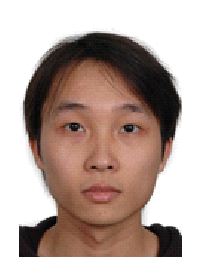
\includegraphics{eps/resume/picture.eps}




\noindent\textbf{教育背景:}\\
(1).~2003年9月$\sim$2007年6月, 中山大学信科院计算机科学与技术专业, 获学士学位。\\
(2).~2007年9月$\sim$2009年6月, 中山大学信科院计算机应用技术专业,硕士研究生。\\

\noindent\textbf{专业经历:} \\
(1).~2007年9月$\sim$至今,中山大学信息与网络中心,研究助理。\\
....................
        %********个人简历
%
\phantomsection

\addcontentsline{toc}{chapter}{\hspace*{0.2cm}致~谢}

\chapter*{ \markboth{致谢}{致谢}}
\vspace{-1cm}\centerline{\xiaoerhao{\hei{致\quad 谢}}}

%\vspace{5mm}{\kai\xiaosihao
论文完成之际,首先感谢中山大学这所高等学府。我在这里学习和生活了六年,这所美丽的学校赋予我许多灵感,也让我有机会结识诸多良师益友。

衷心感谢....

衷心感谢....

衷心感谢....

衷心感谢....

衷心感谢....

最后我要感谢那些在这里不能一一提到的师长、同学和好友,感谢所有帮助和关心过我的人们。谢谢!

%}

%\vspace{2cm}

\hfill {\kai 车春回 \hspace{15mm}

\hfill 2009~年~5~月于康乐园}\hspace{5mm}
        %********致谢
%
\end{document}
